\documentclass[1p]{elsarticle_modified}
%\bibliographystyle{elsarticle-num}

%\usepackage[colorlinks]{hyperref}
%\usepackage{abbrmath_seonhwa} %\Abb, \Ascr, \Acal ,\Abf, \Afrak
\usepackage{amsfonts}
\usepackage{amssymb}
\usepackage{amsmath}
\usepackage{amsthm}
\usepackage{scalefnt}
\usepackage{amsbsy}
\usepackage{kotex}
\usepackage{caption}
\usepackage{subfig}
\usepackage{color}
\usepackage{graphicx}
\usepackage{xcolor} %% white, black, red, green, blue, cyan, magenta, yellow
\usepackage{float}
\usepackage{setspace}
\usepackage{hyperref}

\usepackage{tikz}
\usetikzlibrary{arrows}

\usepackage{multirow}
\usepackage{array} % fixed length table
\usepackage{hhline}

%%%%%%%%%%%%%%%%%%%%%
\makeatletter
\renewcommand*\env@matrix[1][\arraystretch]{%
	\edef\arraystretch{#1}%
	\hskip -\arraycolsep
	\let\@ifnextchar\new@ifnextchar
	\array{*\c@MaxMatrixCols c}}
\makeatother %https://tex.stackexchange.com/questions/14071/how-can-i-increase-the-line-spacing-in-a-matrix
%%%%%%%%%%%%%%%

\usepackage[normalem]{ulem}

\newcommand{\msout}[1]{\ifmmode\text{\sout{\ensuremath{#1}}}\else\sout{#1}\fi}
%SOURCE: \msout is \stkout macro in https://tex.stackexchange.com/questions/20609/strikeout-in-math-mode

\newcommand{\cancel}[1]{
	\ifmmode
	{\color{red}\msout{#1}}
	\else
	{\color{red}\sout{#1}}
	\fi
}

\newcommand{\add}[1]{
	{\color{blue}\uwave{#1}}
}

\newcommand{\replace}[2]{
	\ifmmode
	{\color{red}\msout{#1}}{\color{blue}\uwave{#2}}
	\else
	{\color{red}\sout{#1}}{\color{blue}\uwave{#2}}
	\fi
}

\newcommand{\Sol}{\mathcal{S}} %segment
\newcommand{\D}{D} %diagram
\newcommand{\A}{\mathcal{A}} %arc


%%%%%%%%%%%%%%%%%%%%%%%%%%%%%5 test

\def\sl{\operatorname{\textup{SL}}(2,\Cbb)}
\def\psl{\operatorname{\textup{PSL}}(2,\Cbb)}
\def\quan{\mkern 1mu \triangleright \mkern 1mu}

\theoremstyle{definition}
\newtheorem{thm}{Theorem}[section]
\newtheorem{prop}[thm]{Proposition}
\newtheorem{lem}[thm]{Lemma}
\newtheorem{ques}[thm]{Question}
\newtheorem{cor}[thm]{Corollary}
\newtheorem{defn}[thm]{Definition}
\newtheorem{exam}[thm]{Example}
\newtheorem{rmk}[thm]{Remark}
\newtheorem{alg}[thm]{Algorithm}

\newcommand{\I}{\sqrt{-1}}
\begin{document}

%\begin{frontmatter}
%
%\title{Boundary parabolic representations of knots up to 8 crossings}
%
%%% Group authors per affiliation:
%\author{Yunhi Cho} 
%\address{Department of Mathematics, University of Seoul, Seoul, Korea}
%\ead{yhcho@uos.ac.kr}
%
%
%\author{Seonhwa Kim} %\fnref{s_kim}}
%\address{Center for Geometry and Physics, Institute for Basic Science, Pohang, 37673, Korea}
%\ead{ryeona17@ibs.re.kr}
%
%\author{Hyuk Kim}
%\address{Department of Mathematical Sciences, Seoul National University, Seoul 08826, Korea}
%\ead{hyukkim@snu.ac.kr}
%
%\author{Seokbeom Yoon}
%\address{Department of Mathematical Sciences, Seoul National University, Seoul, 08826,  Korea}
%\ead{sbyoon15@snu.ac.kr}
%
%\begin{abstract}
%We find all boundary parabolic representation of knots up to 8 crossings.
%
%\end{abstract}
%\begin{keyword}
%    \MSC[2010] 57M25 
%\end{keyword}
%
%\end{frontmatter}

%\linenumbers
%\tableofcontents
%
\newcommand\colored[1]{\textcolor{white}{\rule[-0.35ex]{0.8em}{1.4ex}}\kern-0.8em\color{red} #1}%
%\newcommand\colored[1]{\textcolor{white}{ #1}\kern-2.17ex	\textcolor{white}{ #1}\kern-1.81ex	\textcolor{white}{ #1}\kern-2.15ex\color{red}#1	}

{\Large $\underline{12a_{1237}~(K12a_{1237})}$}

\setlength{\tabcolsep}{10pt}
\renewcommand{\arraystretch}{1.6}
\vspace{1cm}\begin{tabular}{m{100pt}>{\centering\arraybackslash}m{274pt}}
\multirow{5}{120pt}{
	\centering
	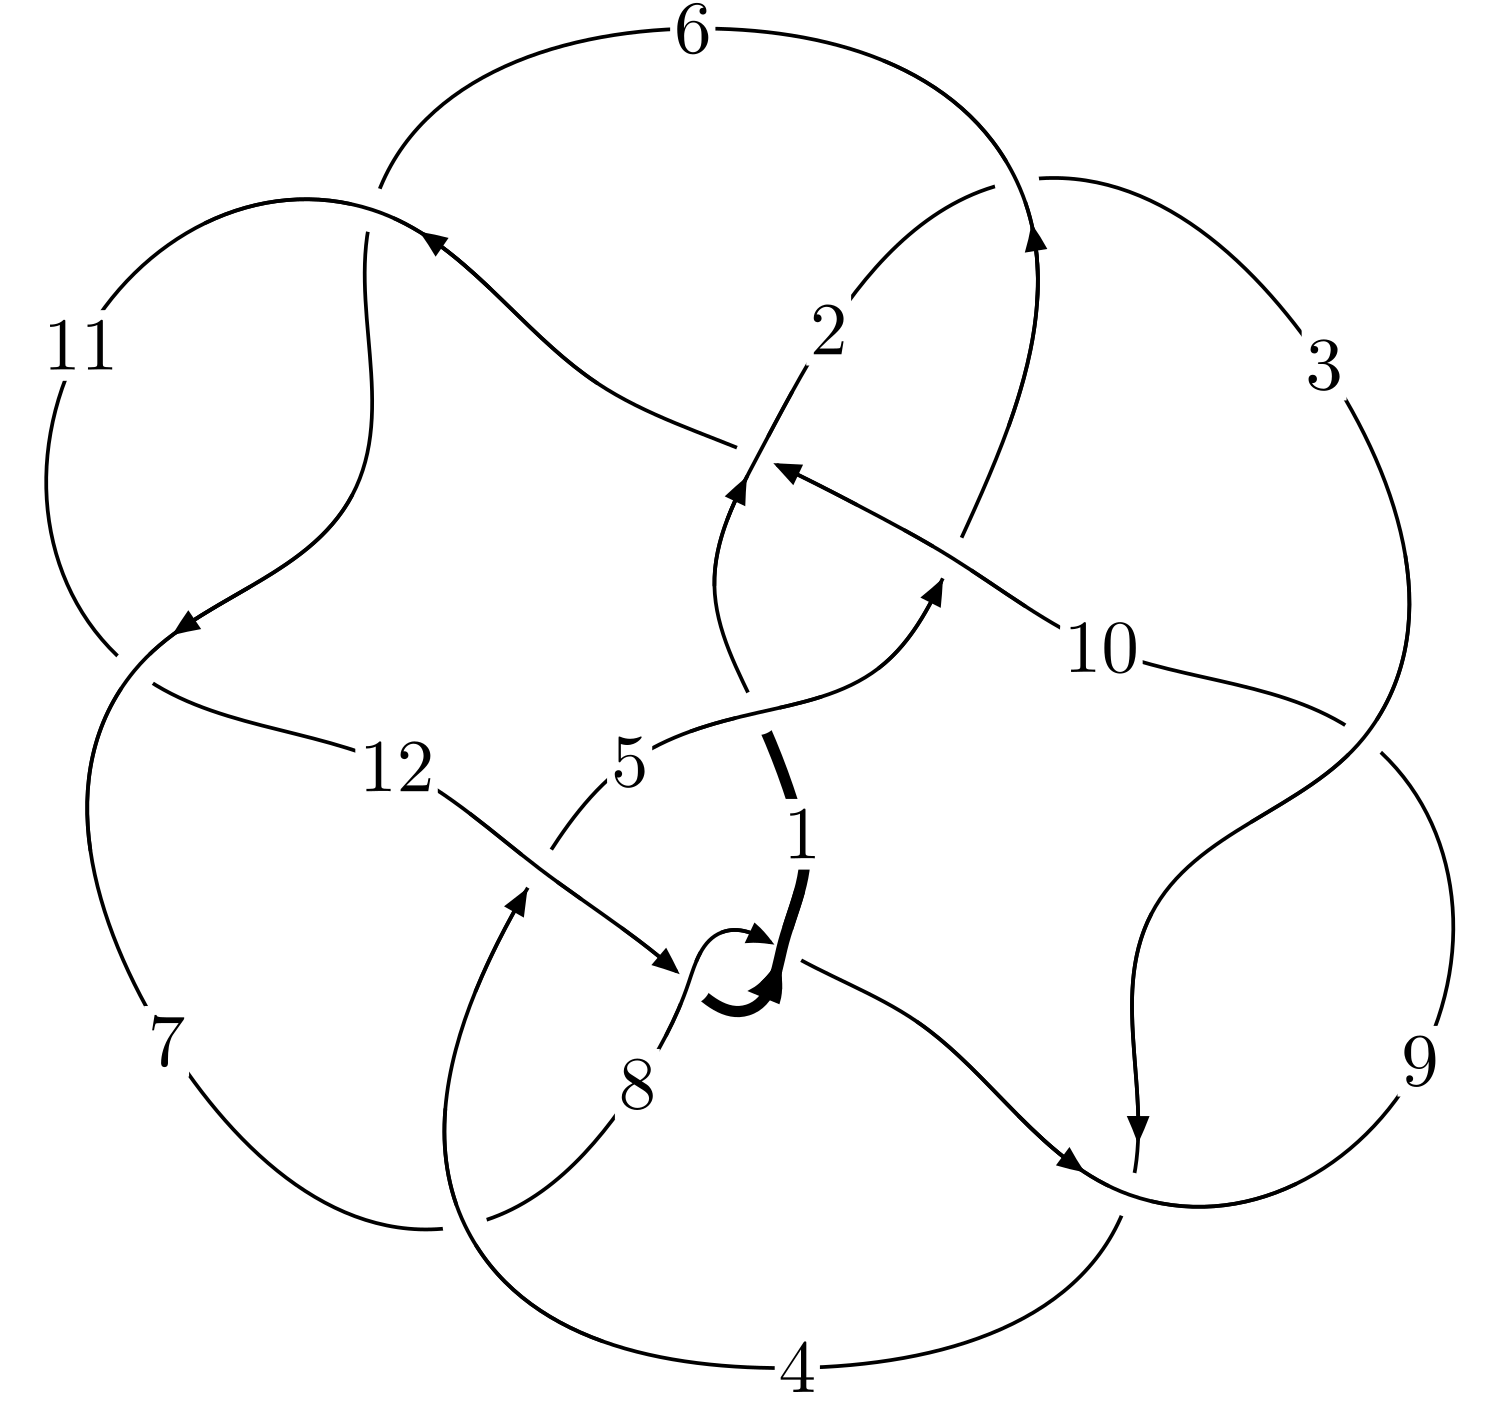
\includegraphics[width=112pt]{../../../GIT/diagram.site/Diagrams/png/2038_12a_1237.png}\\
\ \ \ A knot diagram\footnotemark}&
\allowdisplaybreaks
\textbf{Linearized knot diagam} \\
\cline{2-2}
 &
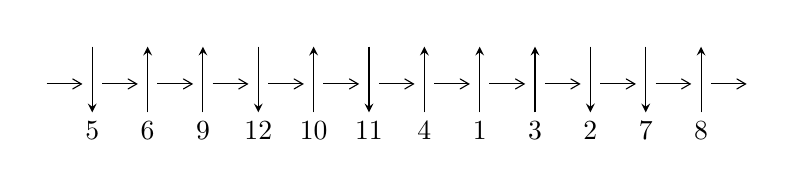
\begin{tikzpicture}[x=20pt, y=17pt]
	% nodes
	\node (C0) at (0, 0) {};
	\node (C1) at (1, 0) {};
	\node (C1U) at (1, +1) {};
	\node (C1D) at (1, -1) {5};

	\node (C2) at (2, 0) {};
	\node (C2U) at (2, +1) {};
	\node (C2D) at (2, -1) {6};

	\node (C3) at (3, 0) {};
	\node (C3U) at (3, +1) {};
	\node (C3D) at (3, -1) {9};

	\node (C4) at (4, 0) {};
	\node (C4U) at (4, +1) {};
	\node (C4D) at (4, -1) {12};

	\node (C5) at (5, 0) {};
	\node (C5U) at (5, +1) {};
	\node (C5D) at (5, -1) {10};

	\node (C6) at (6, 0) {};
	\node (C6U) at (6, +1) {};
	\node (C6D) at (6, -1) {11};

	\node (C7) at (7, 0) {};
	\node (C7U) at (7, +1) {};
	\node (C7D) at (7, -1) {4};

	\node (C8) at (8, 0) {};
	\node (C8U) at (8, +1) {};
	\node (C8D) at (8, -1) {1};

	\node (C9) at (9, 0) {};
	\node (C9U) at (9, +1) {};
	\node (C9D) at (9, -1) {3};

	\node (C10) at (10, 0) {};
	\node (C10U) at (10, +1) {};
	\node (C10D) at (10, -1) {2};

	\node (C11) at (11, 0) {};
	\node (C11U) at (11, +1) {};
	\node (C11D) at (11, -1) {7};

	\node (C12) at (12, 0) {};
	\node (C12U) at (12, +1) {};
	\node (C12D) at (12, -1) {8};
	\node (C13) at (13, 0) {};

	% arrows
	\draw[->,>={angle 60}]
	(C0) edge (C1) (C1) edge (C2) (C2) edge (C3) (C3) edge (C4) (C4) edge (C5) (C5) edge (C6) (C6) edge (C7) (C7) edge (C8) (C8) edge (C9) (C9) edge (C10) (C10) edge (C11) (C11) edge (C12) (C12) edge (C13) ;	\draw[->,>=stealth]
	(C1U) edge (C1D) (C2D) edge (C2U) (C3D) edge (C3U) (C4U) edge (C4D) (C5D) edge (C5U) (C6U) edge (C6D) (C7D) edge (C7U) (C8D) edge (C8U) (C9D) edge (C9U) (C10U) edge (C10D) (C11U) edge (C11D) (C12D) edge (C12U) ;
	\end{tikzpicture} \\
\hhline{~~} \\& 
\textbf{Solving Sequence} \\ \cline{2-2} 
 &
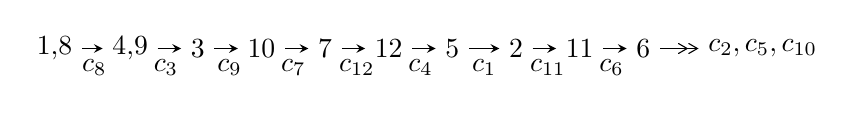
\begin{tikzpicture}[x=23pt, y=7pt]
	% node
	\node (A0) at (-1/8, 0) {1,8};
	\node (A1) at (17/16, 0) {4,9};
	\node (A2) at (17/8, 0) {3};
	\node (A3) at (25/8, 0) {10};
	\node (A4) at (33/8, 0) {7};
	\node (A5) at (41/8, 0) {12};
	\node (A6) at (49/8, 0) {5};
	\node (A7) at (57/8, 0) {2};
	\node (A8) at (65/8, 0) {11};
	\node (A9) at (73/8, 0) {6};
	\node (C1) at (1/2, -1) {$c_{8}$};
	\node (C2) at (13/8, -1) {$c_{3}$};
	\node (C3) at (21/8, -1) {$c_{9}$};
	\node (C4) at (29/8, -1) {$c_{7}$};
	\node (C5) at (37/8, -1) {$c_{12}$};
	\node (C6) at (45/8, -1) {$c_{4}$};
	\node (C7) at (53/8, -1) {$c_{1}$};
	\node (C8) at (61/8, -1) {$c_{11}$};
	\node (C9) at (69/8, -1) {$c_{6}$};
	\node (A10) at (11, 0) {$c_{2},c_{5},c_{10}$};

	% edge
	\draw[->,>=stealth]	
	(A0) edge (A1) (A1) edge (A2) (A2) edge (A3) (A3) edge (A4) (A4) edge (A5) (A5) edge (A6) (A6) edge (A7) (A7) edge (A8) (A8) edge (A9) ;
	\draw[->>,>={angle 60}]	
	(A9) edge (A10);
\end{tikzpicture} \\ 

\end{tabular} \\

\footnotetext{
The image of knot diagram is generated by the software ``\textbf{Draw programme}" developed by Andrew Bartholomew(\url{http://www.layer8.co.uk/maths/draw/index.htm\#Running-draw}), where we modified some parts for our purpose(\url{https://github.com/CATsTAILs/LinksPainter}).
}\phantom \\ \newline 
\centering \textbf{Ideals for irreducible components\footnotemark of $X_{\text{par}}$} 
 
\begin{align*}
I^u_{1}&=\langle 
4.20584\times10^{667} u^{144}+3.01908\times10^{667} u^{143}+\cdots+8.60367\times10^{668} b-7.21833\times10^{670},\\
\phantom{I^u_{1}}&\phantom{= \langle  }-2.18124\times10^{668} u^{144}+1.52575\times10^{670} u^{143}+\cdots+5.53216\times10^{671} a-1.40274\times10^{673},\\
\phantom{I^u_{1}}&\phantom{= \langle  }u^{145}-43 u^{143}+\cdots+14615 u+1286\rangle \\
I^u_{2}&=\langle 
-8.26352\times10^{22} u^{32}-1.84889\times10^{23} u^{31}+\cdots+1.89990\times10^{22} b+1.14959\times10^{24},\\
\phantom{I^u_{2}}&\phantom{= \langle  }-5.63314\times10^{23} u^{32}+8.09901\times10^{22} u^{31}+\cdots+1.32993\times10^{23} a-2.25243\times10^{24},\;u^{33}+u^{32}+\cdots-23 u+7\rangle \\
\\
\end{align*}
\raggedright * 2 irreducible components of $\dim_{\mathbb{C}}=0$, with total 178 representations.\\
\footnotetext{All coefficients of polynomials are rational numbers. But the coefficients are sometimes approximated in decimal forms when there is not enough margin.}
\newpage
\renewcommand{\arraystretch}{1}
\centering \section*{I. $I^u_{1}= \langle 4.21\times10^{667} u^{144}+3.02\times10^{667} u^{143}+\cdots+8.60\times10^{668} b-7.22\times10^{670},\;-2.18\times10^{668} u^{144}+1.53\times10^{670} u^{143}+\cdots+5.53\times10^{671} a-1.40\times10^{673},\;u^{145}-43 u^{143}+\cdots+14615 u+1286 \rangle$}
\flushleft \textbf{(i) Arc colorings}\\
\begin{tabular}{m{7pt} m{180pt} m{7pt} m{180pt} }
\flushright $a_{1}=$&$\begin{pmatrix}0\\u\end{pmatrix}$ \\
\flushright $a_{8}=$&$\begin{pmatrix}1\\0\end{pmatrix}$ \\
\flushright $a_{4}=$&$\begin{pmatrix}0.000394283 u^{144}-0.0275797 u^{143}+\cdots+45.5077 u+25.3561\\-0.0488843 u^{144}-0.0350906 u^{143}+\cdots+1165.03 u+83.8983\end{pmatrix}$ \\
\flushright $a_{9}=$&$\begin{pmatrix}1\\- u^2\end{pmatrix}$ \\
\flushright $a_{3}=$&$\begin{pmatrix}0.116495 u^{144}+0.0671820 u^{143}+\cdots-1522.09 u-94.0097\\-0.134528 u^{144}-0.114336 u^{143}+\cdots+2699.27 u+205.762\end{pmatrix}$ \\
\flushright $a_{10}=$&$\begin{pmatrix}-0.109833 u^{144}-0.104519 u^{143}+\cdots+2368.10 u+190.837\\0.650696 u^{144}+0.595136 u^{143}+\cdots-13544.2 u-1087.67\end{pmatrix}$ \\
\flushright $a_{7}=$&$\begin{pmatrix}-0.174719 u^{144}-0.200942 u^{143}+\cdots+581.947 u+54.6804\\0.0514734 u^{144}+0.0874424 u^{143}+\cdots+1450.89 u+111.392\end{pmatrix}$ \\
\flushright $a_{12}=$&$\begin{pmatrix}- u\\u\end{pmatrix}$ \\
\flushright $a_{5}=$&$\begin{pmatrix}0.0662833 u^{144}+0.0400073 u^{143}+\cdots-932.777 u-55.2379\\-0.114773 u^{144}-0.102678 u^{143}+\cdots+2143.31 u+164.492\end{pmatrix}$ \\
\flushright $a_{2}=$&$\begin{pmatrix}-0.0456777 u^{144}-0.115858 u^{143}+\cdots-172.059 u-13.9622\\0.166438 u^{144}+0.194786 u^{143}+\cdots-2125.71 u-181.588\end{pmatrix}$ \\
\flushright $a_{11}=$&$\begin{pmatrix}-0.179609 u^{144}-0.120283 u^{143}+\cdots+5384.61 u+423.462\\0.188114 u^{144}+0.126517 u^{143}+\cdots-5191.59 u-407.693\end{pmatrix}$ \\
\flushright $a_{6}=$&$\begin{pmatrix}0.151645 u^{144}+0.242592 u^{143}+\cdots-1779.97 u-158.597\\-0.0296550 u^{144}-0.136351 u^{143}+\cdots+97.9273 u+35.0310\end{pmatrix}$\\&\end{tabular}
\flushleft \textbf{(ii) Obstruction class $= -1$}\\~\\
\flushleft \textbf{(iii) Cusp Shapes $= 0.312516 u^{144}-1.83404 u^{143}+\cdots+32956.9 u+2890.88$}\\~\\
\newpage\renewcommand{\arraystretch}{1}
\flushleft \textbf{(iv) u-Polynomials at the component}\newline \\
\begin{tabular}{m{50pt}|m{274pt}}
Crossings & \hspace{64pt}u-Polynomials at each crossing \\
\hline $$\begin{aligned}c_{1}\end{aligned}$$&$\begin{aligned}
&u^{145}-6 u^{144}+\cdots-153422604074 u+82046221679
\end{aligned}$\\
\hline $$\begin{aligned}c_{2}\end{aligned}$$&$\begin{aligned}
&u^{145}- u^{144}+\cdots+525670 u+55949
\end{aligned}$\\
\hline $$\begin{aligned}c_{3},c_{9}\end{aligned}$$&$\begin{aligned}
&u^{145}-5 u^{144}+\cdots+12394259 u+542527
\end{aligned}$\\
\hline $$\begin{aligned}c_{4}\end{aligned}$$&$\begin{aligned}
&u^{145}+10 u^{144}+\cdots-32 u-1
\end{aligned}$\\
\hline $$\begin{aligned}c_{5}\end{aligned}$$&$\begin{aligned}
&u^{145}+3 u^{144}+\cdots-49936 u+13568
\end{aligned}$\\
\hline $$\begin{aligned}c_{6},c_{11}\end{aligned}$$&$\begin{aligned}
&u^{145}- u^{144}+\cdots-134 u+1
\end{aligned}$\\
\hline $$\begin{aligned}c_{7}\end{aligned}$$&$\begin{aligned}
&u^{145}-3 u^{144}+\cdots+1140 u+1117
\end{aligned}$\\
\hline $$\begin{aligned}c_{8},c_{12}\end{aligned}$$&$\begin{aligned}
&u^{145}-43 u^{143}+\cdots+14615 u-1286
\end{aligned}$\\
\hline $$\begin{aligned}c_{10}\end{aligned}$$&$\begin{aligned}
&u^{145}+u^{144}+\cdots-27127 u-9606
\end{aligned}$\\
\hline
\end{tabular}\\~\\
\newpage\renewcommand{\arraystretch}{1}
\flushleft \textbf{(v) Riley Polynomials at the component}\newline \\
\begin{tabular}{m{50pt}|m{274pt}}
Crossings & \hspace{64pt}Riley Polynomials at each crossing \\
\hline $$\begin{aligned}c_{1}\end{aligned}$$&$\begin{aligned}
&y^{145}-84 y^{144}+\cdots+3.96\times10^{23} y-6.73\times10^{21}
\end{aligned}$\\
\hline $$\begin{aligned}c_{2}\end{aligned}$$&$\begin{aligned}
&y^{145}+53 y^{144}+\cdots+51147539762 y-3130290601
\end{aligned}$\\
\hline $$\begin{aligned}c_{3},c_{9}\end{aligned}$$&$\begin{aligned}
&y^{145}+73 y^{144}+\cdots+4228767991095 y-294335545729
\end{aligned}$\\
\hline $$\begin{aligned}c_{4}\end{aligned}$$&$\begin{aligned}
&y^{145}-74 y^{144}+\cdots+198 y-1
\end{aligned}$\\
\hline $$\begin{aligned}c_{5}\end{aligned}$$&$\begin{aligned}
&y^{145}+37 y^{144}+\cdots+1166626560 y-184090624
\end{aligned}$\\
\hline $$\begin{aligned}c_{6},c_{11}\end{aligned}$$&$\begin{aligned}
&y^{145}-131 y^{144}+\cdots+18524 y-1
\end{aligned}$\\
\hline $$\begin{aligned}c_{7}\end{aligned}$$&$\begin{aligned}
&y^{145}+21 y^{144}+\cdots+52277246 y-1247689
\end{aligned}$\\
\hline $$\begin{aligned}c_{8},c_{12}\end{aligned}$$&$\begin{aligned}
&y^{145}-86 y^{144}+\cdots+66531265 y-1653796
\end{aligned}$\\
\hline $$\begin{aligned}c_{10}\end{aligned}$$&$\begin{aligned}
&y^{145}-91 y^{144}+\cdots+5892163597 y-92275236
\end{aligned}$\\
\hline
\end{tabular}\\~\\
\newpage\flushleft \textbf{(vi) Complex Volumes and Cusp Shapes}
$$\begin{array}{c|c|c}  
\text{Solutions to }I^u_{1}& \I (\text{vol} + \sqrt{-1}CS) & \text{Cusp shape}\\
 \hline 
\begin{aligned}
u &= -0.898633 + 0.433440 I \\
a &= \phantom{-}2.04578 - 0.71402 I \\
b &= \phantom{-}0.022491 + 0.409068 I\end{aligned}
 & -9.14402 - 10.24780 I & \phantom{-0.000000 } 0 \\ \hline\begin{aligned}
u &= -0.898633 - 0.433440 I \\
a &= \phantom{-}2.04578 + 0.71402 I \\
b &= \phantom{-}0.022491 - 0.409068 I\end{aligned}
 & -9.14402 + 10.24780 I & \phantom{-0.000000 } 0 \\ \hline\begin{aligned}
u &= -0.073050 + 0.994240 I \\
a &= \phantom{-}0.095870 + 0.255895 I \\
b &= -0.482995 + 0.354364 I\end{aligned}
 & -0.43751 - 3.83986 I & \phantom{-0.000000 } 0 \\ \hline\begin{aligned}
u &= -0.073050 - 0.994240 I \\
a &= \phantom{-}0.095870 - 0.255895 I \\
b &= -0.482995 - 0.354364 I\end{aligned}
 & -0.43751 + 3.83986 I & \phantom{-0.000000 } 0 \\ \hline\begin{aligned}
u &= -0.914397 + 0.386602 I \\
a &= -2.78356 + 0.34868 I \\
b &= \phantom{-}2.04338 - 1.02761 I\end{aligned}
 & -7.57636 - 3.28778 I & \phantom{-0.000000 } 0 \\ \hline\begin{aligned}
u &= -0.914397 - 0.386602 I \\
a &= -2.78356 - 0.34868 I \\
b &= \phantom{-}2.04338 + 1.02761 I\end{aligned}
 & -7.57636 + 3.28778 I & \phantom{-0.000000 } 0 \\ \hline\begin{aligned}
u &= \phantom{-}0.937361 + 0.386454 I \\
a &= -2.15080 - 0.47024 I \\
b &= \phantom{-}0.744495 + 0.535402 I\end{aligned}
 & -3.86981 + 6.90906 I & \phantom{-0.000000 } 0 \\ \hline\begin{aligned}
u &= \phantom{-}0.937361 - 0.386454 I \\
a &= -2.15080 + 0.47024 I \\
b &= \phantom{-}0.744495 - 0.535402 I\end{aligned}
 & -3.86981 - 6.90906 I & \phantom{-0.000000 } 0 \\ \hline\begin{aligned}
u &= -0.475893 + 0.849331 I \\
a &= -0.377473 + 0.252302 I \\
b &= -0.316276 + 1.206530 I\end{aligned}
 & -8.42083 - 4.77169 I & \phantom{-0.000000 } 0 \\ \hline\begin{aligned}
u &= -0.475893 - 0.849331 I \\
a &= -0.377473 - 0.252302 I \\
b &= -0.316276 - 1.206530 I\end{aligned}
 & -8.42083 + 4.77169 I & \phantom{-0.000000 } 0\\
 \hline 
 \end{array}$$\newpage$$\begin{array}{c|c|c}  
\text{Solutions to }I^u_{1}& \I (\text{vol} + \sqrt{-1}CS) & \text{Cusp shape}\\
 \hline 
\begin{aligned}
u &= \phantom{-}0.836276 + 0.480474 I \\
a &= \phantom{-}1.76801 - 0.15769 I \\
b &= -0.951024 - 0.248799 I\end{aligned}
 & -3.17451 + 2.02375 I & \phantom{-0.000000 } 0 \\ \hline\begin{aligned}
u &= \phantom{-}0.836276 - 0.480474 I \\
a &= \phantom{-}1.76801 + 0.15769 I \\
b &= -0.951024 + 0.248799 I\end{aligned}
 & -3.17451 - 2.02375 I & \phantom{-0.000000 } 0 \\ \hline\begin{aligned}
u &= -0.963301\phantom{ +0.000000I} \\
a &= \phantom{-}1.25592\phantom{ +0.000000I} \\
b &= -0.349566\phantom{ +0.000000I}\end{aligned}
 & \phantom{-}1.75193\phantom{ +0.000000I} & \phantom{-0.000000 } 0 \\ \hline\begin{aligned}
u &= \phantom{-}0.848320 + 0.414953 I \\
a &= -1.86905 - 0.89346 I \\
b &= -0.009494 + 0.545050 I\end{aligned}
 & -8.25194 + 1.66327 I & \phantom{-0.000000 } 0 \\ \hline\begin{aligned}
u &= \phantom{-}0.848320 - 0.414953 I \\
a &= -1.86905 + 0.89346 I \\
b &= -0.009494 - 0.545050 I\end{aligned}
 & -8.25194 - 1.66327 I & \phantom{-0.000000 } 0 \\ \hline\begin{aligned}
u &= -1.034370 + 0.211409 I \\
a &= -1.36610 - 0.57021 I \\
b &= \phantom{-}0.887823 - 0.812845 I\end{aligned}
 & \phantom{-}2.98997 - 0.80961 I & \phantom{-0.000000 } 0 \\ \hline\begin{aligned}
u &= -1.034370 - 0.211409 I \\
a &= -1.36610 + 0.57021 I \\
b &= \phantom{-}0.887823 + 0.812845 I\end{aligned}
 & \phantom{-}2.98997 + 0.80961 I & \phantom{-0.000000 } 0 \\ \hline\begin{aligned}
u &= -1.003690 + 0.338682 I \\
a &= \phantom{-}2.79524 - 0.57397 I \\
b &= -1.93910 + 1.12849 I\end{aligned}
 & -7.39281 - 3.03542 I & \phantom{-0.000000 } 0 \\ \hline\begin{aligned}
u &= -1.003690 - 0.338682 I \\
a &= \phantom{-}2.79524 + 0.57397 I \\
b &= -1.93910 - 1.12849 I\end{aligned}
 & -7.39281 + 3.03542 I & \phantom{-0.000000 } 0 \\ \hline\begin{aligned}
u &= \phantom{-}0.906664 + 0.227126 I \\
a &= -2.01583 + 2.24650 I \\
b &= \phantom{-}2.21764 - 2.30679 I\end{aligned}
 & -7.91749 + 8.92787 I & \phantom{-0.000000 } 0\\
 \hline 
 \end{array}$$\newpage$$\begin{array}{c|c|c}  
\text{Solutions to }I^u_{1}& \I (\text{vol} + \sqrt{-1}CS) & \text{Cusp shape}\\
 \hline 
\begin{aligned}
u &= \phantom{-}0.906664 - 0.227126 I \\
a &= -2.01583 - 2.24650 I \\
b &= \phantom{-}2.21764 + 2.30679 I\end{aligned}
 & -7.91749 - 8.92787 I & \phantom{-0.000000 } 0 \\ \hline\begin{aligned}
u &= -0.960213 + 0.462729 I \\
a &= -0.696597 - 0.501211 I \\
b &= \phantom{-}0.772732 - 0.563054 I\end{aligned}
 & \phantom{-}1.32240 - 2.06915 I & \phantom{-0.000000 } 0 \\ \hline\begin{aligned}
u &= -0.960213 - 0.462729 I \\
a &= -0.696597 + 0.501211 I \\
b &= \phantom{-}0.772732 + 0.563054 I\end{aligned}
 & \phantom{-}1.32240 + 2.06915 I & \phantom{-0.000000 } 0 \\ \hline\begin{aligned}
u &= \phantom{-}0.876368 + 0.322529 I \\
a &= \phantom{-}0.005716 - 0.379310 I \\
b &= -0.576803 + 0.637195 I\end{aligned}
 & -2.98776 + 1.27870 I & \phantom{-0.000000 } 0 \\ \hline\begin{aligned}
u &= \phantom{-}0.876368 - 0.322529 I \\
a &= \phantom{-}0.005716 + 0.379310 I \\
b &= -0.576803 - 0.637195 I\end{aligned}
 & -2.98776 - 1.27870 I & \phantom{-0.000000 } 0 \\ \hline\begin{aligned}
u &= \phantom{-}0.933708\phantom{ +0.000000I} \\
a &= \phantom{-}6.36337\phantom{ +0.000000I} \\
b &= -0.420025\phantom{ +0.000000I}\end{aligned}
 & -5.10444\phantom{ +0.000000I} & \phantom{-0.000000 } 0 \\ \hline\begin{aligned}
u &= -0.821912 + 0.689402 I \\
a &= -1.388660 + 0.031507 I \\
b &= -0.129311 - 0.440745 I\end{aligned}
 & -7.46361 - 0.84977 I & \phantom{-0.000000 } 0 \\ \hline\begin{aligned}
u &= -0.821912 - 0.689402 I \\
a &= -1.388660 - 0.031507 I \\
b &= -0.129311 + 0.440745 I\end{aligned}
 & -7.46361 + 0.84977 I & \phantom{-0.000000 } 0 \\ \hline\begin{aligned}
u &= -0.897131 + 0.205839 I \\
a &= -1.50037 + 0.65516 I \\
b &= \phantom{-}0.711261 + 0.549688 I\end{aligned}
 & -0.872138 - 0.966382 I & \phantom{-0.000000 } 0 \\ \hline\begin{aligned}
u &= -0.897131 - 0.205839 I \\
a &= -1.50037 - 0.65516 I \\
b &= \phantom{-}0.711261 - 0.549688 I\end{aligned}
 & -0.872138 + 0.966382 I & \phantom{-0.000000 } 0\\
 \hline 
 \end{array}$$\newpage$$\begin{array}{c|c|c}  
\text{Solutions to }I^u_{1}& \I (\text{vol} + \sqrt{-1}CS) & \text{Cusp shape}\\
 \hline 
\begin{aligned}
u &= -0.839571 + 0.329804 I \\
a &= \phantom{-}2.38943 - 0.64658 I \\
b &= -1.085090 + 0.532412 I\end{aligned}
 & -3.69986 + 2.87607 I & \phantom{-0.000000 } 0 \\ \hline\begin{aligned}
u &= -0.839571 - 0.329804 I \\
a &= \phantom{-}2.38943 + 0.64658 I \\
b &= -1.085090 - 0.532412 I\end{aligned}
 & -3.69986 - 2.87607 I & \phantom{-0.000000 } 0 \\ \hline\begin{aligned}
u &= \phantom{-}1.015250 + 0.435576 I \\
a &= \phantom{-}1.080660 - 0.190779 I \\
b &= -0.990627 + 0.459760 I\end{aligned}
 & -2.96446 + 2.83003 I & \phantom{-0.000000 } 0 \\ \hline\begin{aligned}
u &= \phantom{-}1.015250 - 0.435576 I \\
a &= \phantom{-}1.080660 + 0.190779 I \\
b &= -0.990627 - 0.459760 I\end{aligned}
 & -2.96446 - 2.83003 I & \phantom{-0.000000 } 0 \\ \hline\begin{aligned}
u &= -0.331846 + 1.056180 I \\
a &= -0.227682 + 0.465537 I \\
b &= -0.685480 - 1.094000 I\end{aligned}
 & -10.73840 + 4.63721 I & \phantom{-0.000000 } 0 \\ \hline\begin{aligned}
u &= -0.331846 - 1.056180 I \\
a &= -0.227682 - 0.465537 I \\
b &= -0.685480 + 1.094000 I\end{aligned}
 & -10.73840 - 4.63721 I & \phantom{-0.000000 } 0 \\ \hline\begin{aligned}
u &= -0.848352 + 0.263430 I \\
a &= \phantom{-}0.698771 + 1.023240 I \\
b &= -0.78796 - 1.77851 I\end{aligned}
 & -3.78660 - 5.60011 I & \phantom{-0.000000 } 0 \\ \hline\begin{aligned}
u &= -0.848352 - 0.263430 I \\
a &= \phantom{-}0.698771 - 1.023240 I \\
b &= -0.78796 + 1.77851 I\end{aligned}
 & -3.78660 + 5.60011 I & \phantom{-0.000000 } 0 \\ \hline\begin{aligned}
u &= \phantom{-}0.491158 + 0.735989 I \\
a &= \phantom{-}0.367473 - 0.319825 I \\
b &= -0.021538 + 0.914830 I\end{aligned}
 & -3.89250 + 2.59486 I & \phantom{-0.000000 } 0 \\ \hline\begin{aligned}
u &= \phantom{-}0.491158 - 0.735989 I \\
a &= \phantom{-}0.367473 + 0.319825 I \\
b &= -0.021538 - 0.914830 I\end{aligned}
 & -3.89250 - 2.59486 I & \phantom{-0.000000 } 0\\
 \hline 
 \end{array}$$\newpage$$\begin{array}{c|c|c}  
\text{Solutions to }I^u_{1}& \I (\text{vol} + \sqrt{-1}CS) & \text{Cusp shape}\\
 \hline 
\begin{aligned}
u &= \phantom{-}0.836435 + 0.245410 I \\
a &= -3.46495 - 0.12438 I \\
b &= \phantom{-}2.42765 + 0.29999 I\end{aligned}
 & -8.09693 - 6.69957 I & \phantom{-0.000000 } 0 \\ \hline\begin{aligned}
u &= \phantom{-}0.836435 - 0.245410 I \\
a &= -3.46495 + 0.12438 I \\
b &= \phantom{-}2.42765 - 0.29999 I\end{aligned}
 & -8.09693 + 6.69957 I & \phantom{-0.000000 } 0 \\ \hline\begin{aligned}
u &= -0.144921 + 1.122370 I \\
a &= -0.004153 - 0.339743 I \\
b &= \phantom{-}0.613411 + 1.178640 I\end{aligned}
 & -11.26920 + 4.43339 I & \phantom{-0.000000 } 0 \\ \hline\begin{aligned}
u &= -0.144921 - 1.122370 I \\
a &= -0.004153 + 0.339743 I \\
b &= \phantom{-}0.613411 - 1.178640 I\end{aligned}
 & -11.26920 - 4.43339 I & \phantom{-0.000000 } 0 \\ \hline\begin{aligned}
u &= \phantom{-}0.868225\phantom{ +0.000000I} \\
a &= \phantom{-}5.44804\phantom{ +0.000000I} \\
b &= \phantom{-}0.110422\phantom{ +0.000000I}\end{aligned}
 & -5.23111\phantom{ +0.000000I} & \phantom{-0.000000 } 0 \\ \hline\begin{aligned}
u &= -1.115650 + 0.205892 I \\
a &= \phantom{-}1.59095 - 0.40657 I \\
b &= -1.10848 + 1.45346 I\end{aligned}
 & \phantom{-}0.51133 - 5.86067 I & \phantom{-0.000000 } 0 \\ \hline\begin{aligned}
u &= -1.115650 - 0.205892 I \\
a &= \phantom{-}1.59095 + 0.40657 I \\
b &= -1.10848 - 1.45346 I\end{aligned}
 & \phantom{-}0.51133 + 5.86067 I & \phantom{-0.000000 } 0 \\ \hline\begin{aligned}
u &= -0.863460\phantom{ +0.000000I} \\
a &= -3.98667\phantom{ +0.000000I} \\
b &= \phantom{-}0.266556\phantom{ +0.000000I}\end{aligned}
 & -0.389672\phantom{ +0.000000I} & \phantom{-0.000000 } 0 \\ \hline\begin{aligned}
u &= \phantom{-}0.384602 + 0.771833 I \\
a &= -0.524388 + 0.192221 I \\
b &= -0.624082 + 0.685763 I\end{aligned}
 & -5.27893 - 2.49198 I & \phantom{-0.000000 } 0 \\ \hline\begin{aligned}
u &= \phantom{-}0.384602 - 0.771833 I \\
a &= -0.524388 - 0.192221 I \\
b &= -0.624082 - 0.685763 I\end{aligned}
 & -5.27893 + 2.49198 I & \phantom{-0.000000 } 0\\
 \hline 
 \end{array}$$\newpage$$\begin{array}{c|c|c}  
\text{Solutions to }I^u_{1}& \I (\text{vol} + \sqrt{-1}CS) & \text{Cusp shape}\\
 \hline 
\begin{aligned}
u &= -1.117890 + 0.257186 I \\
a &= \phantom{-}1.182530 + 0.496514 I \\
b &= -0.433470 + 0.529528 I\end{aligned}
 & \phantom{-}1.64618 - 0.93659 I & \phantom{-0.000000 } 0 \\ \hline\begin{aligned}
u &= -1.117890 - 0.257186 I \\
a &= \phantom{-}1.182530 - 0.496514 I \\
b &= -0.433470 - 0.529528 I\end{aligned}
 & \phantom{-}1.64618 + 0.93659 I & \phantom{-0.000000 } 0 \\ \hline\begin{aligned}
u &= \phantom{-}1.138700 + 0.178079 I \\
a &= -1.46336 - 0.00916 I \\
b &= \phantom{-}1.117940 + 0.749491 I\end{aligned}
 & \phantom{-}4.54964 + 2.34980 I & \phantom{-0.000000 } 0 \\ \hline\begin{aligned}
u &= \phantom{-}1.138700 - 0.178079 I \\
a &= -1.46336 + 0.00916 I \\
b &= \phantom{-}1.117940 - 0.749491 I\end{aligned}
 & \phantom{-}4.54964 - 2.34980 I & \phantom{-0.000000 } 0 \\ \hline\begin{aligned}
u &= -1.113680 + 0.307956 I \\
a &= -0.475025 - 1.248050 I \\
b &= \phantom{-}0.72223 + 1.32017 I\end{aligned}
 & -2.67518 - 5.53153 I & \phantom{-0.000000 } 0 \\ \hline\begin{aligned}
u &= -1.113680 - 0.307956 I \\
a &= -0.475025 + 1.248050 I \\
b &= \phantom{-}0.72223 - 1.32017 I\end{aligned}
 & -2.67518 + 5.53153 I & \phantom{-0.000000 } 0 \\ \hline\begin{aligned}
u &= \phantom{-}1.039010 + 0.517552 I \\
a &= \phantom{-}1.307890 - 0.431307 I \\
b &= -0.877573 - 1.049230 I\end{aligned}
 & -3.36739 + 7.26851 I & \phantom{-0.000000 } 0 \\ \hline\begin{aligned}
u &= \phantom{-}1.039010 - 0.517552 I \\
a &= \phantom{-}1.307890 + 0.431307 I \\
b &= -0.877573 + 1.049230 I\end{aligned}
 & -3.36739 - 7.26851 I & \phantom{-0.000000 } 0 \\ \hline\begin{aligned}
u &= \phantom{-}0.782201 + 0.292217 I \\
a &= \phantom{-}0.185923 - 0.605067 I \\
b &= -0.151287 - 1.391030 I\end{aligned}
 & -8.61903 + 1.53554 I & \phantom{-0.000000 } 0 \\ \hline\begin{aligned}
u &= \phantom{-}0.782201 - 0.292217 I \\
a &= \phantom{-}0.185923 + 0.605067 I \\
b &= -0.151287 + 1.391030 I\end{aligned}
 & -8.61903 - 1.53554 I & \phantom{-0.000000 } 0\\
 \hline 
 \end{array}$$\newpage$$\begin{array}{c|c|c}  
\text{Solutions to }I^u_{1}& \I (\text{vol} + \sqrt{-1}CS) & \text{Cusp shape}\\
 \hline 
\begin{aligned}
u &= \phantom{-}0.062853 + 0.830271 I \\
a &= -0.277114 + 0.555346 I \\
b &= \phantom{-}0.869667 + 0.872090 I\end{aligned}
 & -6.08621 + 8.40067 I & \phantom{-0.000000 } 0 \\ \hline\begin{aligned}
u &= \phantom{-}0.062853 - 0.830271 I \\
a &= -0.277114 - 0.555346 I \\
b &= \phantom{-}0.869667 - 0.872090 I\end{aligned}
 & -6.08621 - 8.40067 I & \phantom{-0.000000 } 0 \\ \hline\begin{aligned}
u &= \phantom{-}1.120600 + 0.358973 I \\
a &= -1.71531 + 0.77940 I \\
b &= \phantom{-}0.733277 + 0.838598 I\end{aligned}
 & -2.41047 + 1.27904 I & \phantom{-0.000000 } 0 \\ \hline\begin{aligned}
u &= \phantom{-}1.120600 - 0.358973 I \\
a &= -1.71531 - 0.77940 I \\
b &= \phantom{-}0.733277 - 0.838598 I\end{aligned}
 & -2.41047 - 1.27904 I & \phantom{-0.000000 } 0 \\ \hline\begin{aligned}
u &= -0.645790 + 0.476309 I \\
a &= \phantom{-}0.466016 - 0.865417 I \\
b &= \phantom{-}0.072640 - 1.236160 I\end{aligned}
 & -9.88006 + 6.43655 I & \phantom{-0.000000 } 0 \\ \hline\begin{aligned}
u &= -0.645790 - 0.476309 I \\
a &= \phantom{-}0.466016 + 0.865417 I \\
b &= \phantom{-}0.072640 + 1.236160 I\end{aligned}
 & -9.88006 - 6.43655 I & \phantom{-0.000000 } 0 \\ \hline\begin{aligned}
u &= \phantom{-}0.774380 + 0.053858 I \\
a &= \phantom{-}2.95434 + 0.15321 I \\
b &= -1.258710 + 0.574099 I\end{aligned}
 & -4.72280 - 0.62776 I & \phantom{-0.000000 } 0 \\ \hline\begin{aligned}
u &= \phantom{-}0.774380 - 0.053858 I \\
a &= \phantom{-}2.95434 - 0.15321 I \\
b &= -1.258710 - 0.574099 I\end{aligned}
 & -4.72280 + 0.62776 I & \phantom{-0.000000 } 0 \\ \hline\begin{aligned}
u &= \phantom{-}0.158103 + 1.213980 I \\
a &= \phantom{-}0.081824 + 0.301611 I \\
b &= \phantom{-}0.624654 - 1.104520 I\end{aligned}
 & -12.3347 - 13.4249 I & \phantom{-0.000000 } 0 \\ \hline\begin{aligned}
u &= \phantom{-}0.158103 - 1.213980 I \\
a &= \phantom{-}0.081824 - 0.301611 I \\
b &= \phantom{-}0.624654 + 1.104520 I\end{aligned}
 & -12.3347 + 13.4249 I & \phantom{-0.000000 } 0\\
 \hline 
 \end{array}$$\newpage$$\begin{array}{c|c|c}  
\text{Solutions to }I^u_{1}& \I (\text{vol} + \sqrt{-1}CS) & \text{Cusp shape}\\
 \hline 
\begin{aligned}
u &= \phantom{-}1.237180 + 0.077493 I \\
a &= \phantom{-}0.846736 - 0.280248 I \\
b &= -0.698183 - 0.515999 I\end{aligned}
 & \phantom{-}3.31935 - 4.02427 I & \phantom{-0.000000 } 0 \\ \hline\begin{aligned}
u &= \phantom{-}1.237180 - 0.077493 I \\
a &= \phantom{-}0.846736 + 0.280248 I \\
b &= -0.698183 + 0.515999 I\end{aligned}
 & \phantom{-}3.31935 + 4.02427 I & \phantom{-0.000000 } 0 \\ \hline\begin{aligned}
u &= -1.175410 + 0.450966 I \\
a &= \phantom{-}1.152680 + 0.175544 I \\
b &= -0.708836 + 1.198700 I\end{aligned}
 & -2.44550 - 5.88329 I & \phantom{-0.000000 } 0 \\ \hline\begin{aligned}
u &= -1.175410 - 0.450966 I \\
a &= \phantom{-}1.152680 - 0.175544 I \\
b &= -0.708836 - 1.198700 I\end{aligned}
 & -2.44550 + 5.88329 I & \phantom{-0.000000 } 0 \\ \hline\begin{aligned}
u &= \phantom{-}1.204180 + 0.420425 I \\
a &= -1.49791 - 0.20124 I \\
b &= \phantom{-}1.11052 + 1.10939 I\end{aligned}
 & \phantom{-}3.24137 + 5.64934 I & \phantom{-0.000000 } 0 \\ \hline\begin{aligned}
u &= \phantom{-}1.204180 - 0.420425 I \\
a &= -1.49791 + 0.20124 I \\
b &= \phantom{-}1.11052 - 1.10939 I\end{aligned}
 & \phantom{-}3.24137 - 5.64934 I & \phantom{-0.000000 } 0 \\ \hline\begin{aligned}
u &= \phantom{-}1.223000 + 0.368504 I \\
a &= -0.570052 - 0.298849 I \\
b &= \phantom{-}0.358043 + 1.108290 I\end{aligned}
 & \phantom{-}1.98338 + 4.93352 I & \phantom{-0.000000 } 0 \\ \hline\begin{aligned}
u &= \phantom{-}1.223000 - 0.368504 I \\
a &= -0.570052 + 0.298849 I \\
b &= \phantom{-}0.358043 - 1.108290 I\end{aligned}
 & \phantom{-}1.98338 - 4.93352 I & \phantom{-0.000000 } 0 \\ \hline\begin{aligned}
u &= \phantom{-}1.285900 + 0.021169 I \\
a &= -0.188657 - 0.967948 I \\
b &= -0.154303 + 0.244970 I\end{aligned}
 & -4.00952 - 1.21936 I & \phantom{-0.000000 } 0 \\ \hline\begin{aligned}
u &= \phantom{-}1.285900 - 0.021169 I \\
a &= -0.188657 + 0.967948 I \\
b &= -0.154303 - 0.244970 I\end{aligned}
 & -4.00952 + 1.21936 I & \phantom{-0.000000 } 0\\
 \hline 
 \end{array}$$\newpage$$\begin{array}{c|c|c}  
\text{Solutions to }I^u_{1}& \I (\text{vol} + \sqrt{-1}CS) & \text{Cusp shape}\\
 \hline 
\begin{aligned}
u &= \phantom{-}0.607686 + 0.374263 I \\
a &= -0.256818 + 0.126683 I \\
b &= \phantom{-}0.378365 - 1.347710 I\end{aligned}
 & -4.85534 - 3.53482 I & \phantom{-0.000000 } 0 \\ \hline\begin{aligned}
u &= \phantom{-}0.607686 - 0.374263 I \\
a &= -0.256818 - 0.126683 I \\
b &= \phantom{-}0.378365 + 1.347710 I\end{aligned}
 & -4.85534 + 3.53482 I & \phantom{-0.000000 } 0 \\ \hline\begin{aligned}
u &= \phantom{-}0.006194 + 1.296310 I \\
a &= -0.194923 - 0.134528 I \\
b &= -0.405453 + 1.086060 I\end{aligned}
 & -10.03280 - 3.13108 I & \phantom{-0.000000 } 0 \\ \hline\begin{aligned}
u &= \phantom{-}0.006194 - 1.296310 I \\
a &= -0.194923 + 0.134528 I \\
b &= -0.405453 - 1.086060 I\end{aligned}
 & -10.03280 + 3.13108 I & \phantom{-0.000000 } 0 \\ \hline\begin{aligned}
u &= -1.29995\phantom{ +0.000000I} \\
a &= \phantom{-}0.998521\phantom{ +0.000000I} \\
b &= -1.05683\phantom{ +0.000000I}\end{aligned}
 & \phantom{-}0.925547\phantom{ +0.000000I} & \phantom{-0.000000 } 0 \\ \hline\begin{aligned}
u &= \phantom{-}1.185940 + 0.534791 I \\
a &= \phantom{-}0.997722 - 0.001953 I \\
b &= -0.933561 + 0.035527 I\end{aligned}
 & -2.95837 + 2.92828 I & \phantom{-0.000000 } 0 \\ \hline\begin{aligned}
u &= \phantom{-}1.185940 - 0.534791 I \\
a &= \phantom{-}0.997722 + 0.001953 I \\
b &= -0.933561 - 0.035527 I\end{aligned}
 & -2.95837 - 2.92828 I & \phantom{-0.000000 } 0 \\ \hline\begin{aligned}
u &= -1.250980 + 0.457236 I \\
a &= -1.62475 - 0.23683 I \\
b &= \phantom{-}0.98700 - 1.03739 I\end{aligned}
 & -2.20657 - 12.99010 I & \phantom{-0.000000 } 0 \\ \hline\begin{aligned}
u &= -1.250980 - 0.457236 I \\
a &= -1.62475 + 0.23683 I \\
b &= \phantom{-}0.98700 + 1.03739 I\end{aligned}
 & -2.20657 + 12.99010 I & \phantom{-0.000000 } 0 \\ \hline\begin{aligned}
u &= \phantom{-}1.180260 + 0.645438 I \\
a &= -0.095049 + 0.660989 I \\
b &= \phantom{-}0.419081 - 0.686751 I\end{aligned}
 & -2.94867 - 3.33911 I & \phantom{-0.000000 } 0\\
 \hline 
 \end{array}$$\newpage$$\begin{array}{c|c|c}  
\text{Solutions to }I^u_{1}& \I (\text{vol} + \sqrt{-1}CS) & \text{Cusp shape}\\
 \hline 
\begin{aligned}
u &= \phantom{-}1.180260 - 0.645438 I \\
a &= -0.095049 - 0.660989 I \\
b &= \phantom{-}0.419081 + 0.686751 I\end{aligned}
 & -2.94867 + 3.33911 I & \phantom{-0.000000 } 0 \\ \hline\begin{aligned}
u &= -1.288430 + 0.393723 I \\
a &= \phantom{-}1.145800 + 0.062438 I \\
b &= -0.916583 + 0.507128 I\end{aligned}
 & \phantom{-}4.10046 - 1.25400 I & \phantom{-0.000000 } 0 \\ \hline\begin{aligned}
u &= -1.288430 - 0.393723 I \\
a &= \phantom{-}1.145800 - 0.062438 I \\
b &= -0.916583 - 0.507128 I\end{aligned}
 & \phantom{-}4.10046 + 1.25400 I & \phantom{-0.000000 } 0 \\ \hline\begin{aligned}
u &= -1.302400 + 0.377450 I \\
a &= -1.38469 + 0.64761 I \\
b &= \phantom{-}1.16529 - 1.16618 I\end{aligned}
 & \phantom{-}1.30978 - 6.31424 I & \phantom{-0.000000 } 0 \\ \hline\begin{aligned}
u &= -1.302400 - 0.377450 I \\
a &= -1.38469 - 0.64761 I \\
b &= \phantom{-}1.16529 + 1.16618 I\end{aligned}
 & \phantom{-}1.30978 + 6.31424 I & \phantom{-0.000000 } 0 \\ \hline\begin{aligned}
u &= \phantom{-}1.270290 + 0.475410 I \\
a &= \phantom{-}1.144090 - 0.252910 I \\
b &= -0.870719 - 0.767104 I\end{aligned}
 & \phantom{-}3.61384 + 8.84204 I & \phantom{-0.000000 } 0 \\ \hline\begin{aligned}
u &= \phantom{-}1.270290 - 0.475410 I \\
a &= \phantom{-}1.144090 + 0.252910 I \\
b &= -0.870719 + 0.767104 I\end{aligned}
 & \phantom{-}3.61384 - 8.84204 I & \phantom{-0.000000 } 0 \\ \hline\begin{aligned}
u &= -0.013019 + 0.638822 I \\
a &= \phantom{-}0.456205 - 0.130262 I \\
b &= \phantom{-}0.395363 - 0.697509 I\end{aligned}
 & -0.26999 - 1.63427 I & \phantom{-0.000000 -}0. + 5.25975 I \\ \hline\begin{aligned}
u &= -0.013019 - 0.638822 I \\
a &= \phantom{-}0.456205 + 0.130262 I \\
b &= \phantom{-}0.395363 + 0.697509 I\end{aligned}
 & -0.26999 + 1.63427 I & \phantom{-0.000000 } 0. - 5.25975 I \\ \hline\begin{aligned}
u &= \phantom{-}1.324790 + 0.345426 I \\
a &= \phantom{-}1.48774 + 1.13838 I \\
b &= -1.18572 - 1.94164 I\end{aligned}
 & -2.93740 + 8.61628 I & \phantom{-0.000000 } 0\\
 \hline 
 \end{array}$$\newpage$$\begin{array}{c|c|c}  
\text{Solutions to }I^u_{1}& \I (\text{vol} + \sqrt{-1}CS) & \text{Cusp shape}\\
 \hline 
\begin{aligned}
u &= \phantom{-}1.324790 - 0.345426 I \\
a &= \phantom{-}1.48774 - 1.13838 I \\
b &= -1.18572 + 1.94164 I\end{aligned}
 & -2.93740 - 8.61628 I & \phantom{-0.000000 } 0 \\ \hline\begin{aligned}
u &= -1.226150 + 0.625099 I \\
a &= \phantom{-}1.60290 - 0.18141 I \\
b &= -1.23535 + 1.29765 I\end{aligned}
 & -7.89645 - 10.62710 I & \phantom{-0.000000 } 0 \\ \hline\begin{aligned}
u &= -1.226150 - 0.625099 I \\
a &= \phantom{-}1.60290 + 0.18141 I \\
b &= -1.23535 - 1.29765 I\end{aligned}
 & -7.89645 + 10.62710 I & \phantom{-0.000000 } 0 \\ \hline\begin{aligned}
u &= -0.117272 + 0.603896 I \\
a &= -0.90517 - 1.13829 I \\
b &= -0.538411 - 0.718761 I\end{aligned}
 & -5.49473 + 1.74369 I & -5.85606 - 4.80060 I \\ \hline\begin{aligned}
u &= -0.117272 - 0.603896 I \\
a &= -0.90517 + 1.13829 I \\
b &= -0.538411 + 0.718761 I\end{aligned}
 & -5.49473 - 1.74369 I & -5.85606 + 4.80060 I \\ \hline\begin{aligned}
u &= \phantom{-}0.113489 + 1.387080 I \\
a &= \phantom{-}0.092029 - 0.253063 I \\
b &= -0.091131 + 0.767086 I\end{aligned}
 & -5.82799 - 0.68385 I & \phantom{-0.000000 } 0 \\ \hline\begin{aligned}
u &= \phantom{-}0.113489 - 1.387080 I \\
a &= \phantom{-}0.092029 + 0.253063 I \\
b &= -0.091131 - 0.767086 I\end{aligned}
 & -5.82799 + 0.68385 I & \phantom{-0.000000 } 0 \\ \hline\begin{aligned}
u &= -1.246240 + 0.646134 I \\
a &= -0.334713 - 0.260613 I \\
b &= \phantom{-}0.509481 - 0.280336 I\end{aligned}
 & \phantom{-}1.97387 - 3.04466 I & \phantom{-0.000000 } 0 \\ \hline\begin{aligned}
u &= -1.246240 - 0.646134 I \\
a &= -0.334713 + 0.260613 I \\
b &= \phantom{-}0.509481 + 0.280336 I\end{aligned}
 & \phantom{-}1.97387 + 3.04466 I & \phantom{-0.000000 } 0 \\ \hline\begin{aligned}
u &= \phantom{-}1.154430 + 0.807051 I \\
a &= -1.084390 + 0.241121 I \\
b &= \phantom{-}1.129930 + 0.604981 I\end{aligned}
 & -1.76551 + 2.91986 I & \phantom{-0.000000 } 0\\
 \hline 
 \end{array}$$\newpage$$\begin{array}{c|c|c}  
\text{Solutions to }I^u_{1}& \I (\text{vol} + \sqrt{-1}CS) & \text{Cusp shape}\\
 \hline 
\begin{aligned}
u &= \phantom{-}1.154430 - 0.807051 I \\
a &= -1.084390 - 0.241121 I \\
b &= \phantom{-}1.129930 - 0.604981 I\end{aligned}
 & -1.76551 - 2.91986 I & \phantom{-0.000000 } 0 \\ \hline\begin{aligned}
u &= -0.057357 + 0.586543 I \\
a &= -0.77673 - 1.35333 I \\
b &= \phantom{-}1.000910 - 0.724742 I\end{aligned}
 & -5.62610 + 2.08118 I & -5.84811 - 3.37812 I \\ \hline\begin{aligned}
u &= -0.057357 - 0.586543 I \\
a &= -0.77673 + 1.35333 I \\
b &= \phantom{-}1.000910 + 0.724742 I\end{aligned}
 & -5.62610 - 2.08118 I & -5.84811 + 3.37812 I \\ \hline\begin{aligned}
u &= -1.29883 + 0.59802 I \\
a &= -1.68501 + 0.26859 I \\
b &= \phantom{-}1.18761 - 1.25695 I\end{aligned}
 & -7.67746 - 10.47000 I & \phantom{-0.000000 } 0 \\ \hline\begin{aligned}
u &= -1.29883 - 0.59802 I \\
a &= -1.68501 - 0.26859 I \\
b &= \phantom{-}1.18761 + 1.25695 I\end{aligned}
 & -7.67746 + 10.47000 I & \phantom{-0.000000 } 0 \\ \hline\begin{aligned}
u &= \phantom{-}1.28284 + 0.67452 I \\
a &= \phantom{-}1.252440 + 0.041811 I \\
b &= -0.910566 - 0.810359 I\end{aligned}
 & -2.42139 + 7.59080 I & \phantom{-0.000000 } 0 \\ \hline\begin{aligned}
u &= \phantom{-}1.28284 - 0.67452 I \\
a &= \phantom{-}1.252440 - 0.041811 I \\
b &= -0.910566 + 0.810359 I\end{aligned}
 & -2.42139 - 7.59080 I & \phantom{-0.000000 } 0 \\ \hline\begin{aligned}
u &= -0.506710 + 0.172553 I \\
a &= -0.21425 + 2.51407 I \\
b &= -0.50236 - 2.06517 I\end{aligned}
 & -8.92961 + 0.23426 I & -9.16694 + 3.14387 I \\ \hline\begin{aligned}
u &= -0.506710 - 0.172553 I \\
a &= -0.21425 - 2.51407 I \\
b &= -0.50236 + 2.06517 I\end{aligned}
 & -8.92961 - 0.23426 I & -9.16694 - 3.14387 I \\ \hline\begin{aligned}
u &= -0.403234 + 0.350283 I \\
a &= \phantom{-}0.53928 - 2.21759 I \\
b &= \phantom{-}0.40326 + 1.75560 I\end{aligned}
 & -8.80263 - 0.13299 I & -8.04077 + 0.88602 I\\
 \hline 
 \end{array}$$\newpage$$\begin{array}{c|c|c}  
\text{Solutions to }I^u_{1}& \I (\text{vol} + \sqrt{-1}CS) & \text{Cusp shape}\\
 \hline 
\begin{aligned}
u &= -0.403234 - 0.350283 I \\
a &= \phantom{-}0.53928 + 2.21759 I \\
b &= \phantom{-}0.40326 - 1.75560 I\end{aligned}
 & -8.80263 + 0.13299 I & -8.04077 - 0.88602 I \\ \hline\begin{aligned}
u &= \phantom{-}1.32675 + 0.63625 I \\
a &= -1.53051 - 0.23758 I \\
b &= \phantom{-}1.15204 + 1.31248 I\end{aligned}
 & -8.6793 + 19.8625 I & \phantom{-0.000000 } 0 \\ \hline\begin{aligned}
u &= \phantom{-}1.32675 - 0.63625 I \\
a &= -1.53051 + 0.23758 I \\
b &= \phantom{-}1.15204 - 1.31248 I\end{aligned}
 & -8.6793 - 19.8625 I & \phantom{-0.000000 } 0 \\ \hline\begin{aligned}
u &= -1.29731 + 0.71010 I \\
a &= \phantom{-}1.278090 + 0.023946 I \\
b &= -1.15402 + 0.88275 I\end{aligned}
 & -1.81745 - 13.82520 I & \phantom{-0.000000 } 0 \\ \hline\begin{aligned}
u &= -1.29731 - 0.71010 I \\
a &= \phantom{-}1.278090 - 0.023946 I \\
b &= -1.15402 - 0.88275 I\end{aligned}
 & -1.81745 + 13.82520 I & \phantom{-0.000000 } 0 \\ \hline\begin{aligned}
u &= \phantom{-}0.056774 + 0.498235 I \\
a &= \phantom{-}1.05776 - 1.07957 I \\
b &= -0.236580 - 0.572621 I\end{aligned}
 & -1.41654 - 1.54812 I & -3.80548 - 0.14559 I \\ \hline\begin{aligned}
u &= \phantom{-}0.056774 - 0.498235 I \\
a &= \phantom{-}1.05776 + 1.07957 I \\
b &= -0.236580 + 0.572621 I\end{aligned}
 & -1.41654 + 1.54812 I & -3.80548 + 0.14559 I \\ \hline\begin{aligned}
u &= -1.37810 + 0.69770 I \\
a &= -0.973448 + 0.212761 I \\
b &= \phantom{-}0.814170 - 0.929985 I\end{aligned}
 & -1.54230 - 6.50583 I & \phantom{-0.000000 } 0 \\ \hline\begin{aligned}
u &= -1.37810 - 0.69770 I \\
a &= -0.973448 - 0.212761 I \\
b &= \phantom{-}0.814170 + 0.929985 I\end{aligned}
 & -1.54230 + 6.50583 I & \phantom{-0.000000 } 0 \\ \hline\begin{aligned}
u &= \phantom{-}1.38713 + 0.68390 I \\
a &= \phantom{-}1.161990 + 0.260414 I \\
b &= -0.86430 - 1.33623 I\end{aligned}
 & -5.82548 + 10.01670 I & \phantom{-0.000000 } 0\\
 \hline 
 \end{array}$$\newpage$$\begin{array}{c|c|c}  
\text{Solutions to }I^u_{1}& \I (\text{vol} + \sqrt{-1}CS) & \text{Cusp shape}\\
 \hline 
\begin{aligned}
u &= \phantom{-}1.38713 - 0.68390 I \\
a &= \phantom{-}1.161990 - 0.260414 I \\
b &= -0.86430 + 1.33623 I\end{aligned}
 & -5.82548 - 10.01670 I & \phantom{-0.000000 } 0 \\ \hline\begin{aligned}
u &= \phantom{-}1.16376 + 1.03937 I \\
a &= -0.633877 + 0.373111 I \\
b &= \phantom{-}0.936357 + 0.080902 I\end{aligned}
 & -2.42551 + 4.70764 I & \phantom{-0.000000 } 0 \\ \hline\begin{aligned}
u &= \phantom{-}1.16376 - 1.03937 I \\
a &= -0.633877 - 0.373111 I \\
b &= \phantom{-}0.936357 - 0.080902 I\end{aligned}
 & -2.42551 - 4.70764 I & \phantom{-0.000000 } 0 \\ \hline\begin{aligned}
u &= -0.46315 + 1.50664 I \\
a &= \phantom{-}0.096500 + 0.334106 I \\
b &= -0.474727 - 0.495902 I\end{aligned}
 & -4.81508 + 6.58039 I & \phantom{-0.000000 } 0 \\ \hline\begin{aligned}
u &= -0.46315 - 1.50664 I \\
a &= \phantom{-}0.096500 - 0.334106 I \\
b &= -0.474727 + 0.495902 I\end{aligned}
 & -4.81508 - 6.58039 I & \phantom{-0.000000 } 0 \\ \hline\begin{aligned}
u &= -1.45498 + 0.78984 I \\
a &= -0.598174 + 0.231653 I \\
b &= \phantom{-}0.129837 - 0.483813 I\end{aligned}
 & -5.65492 - 4.02160 I & \phantom{-0.000000 } 0 \\ \hline\begin{aligned}
u &= -1.45498 - 0.78984 I \\
a &= -0.598174 - 0.231653 I \\
b &= \phantom{-}0.129837 + 0.483813 I\end{aligned}
 & -5.65492 + 4.02160 I & \phantom{-0.000000 } 0 \\ \hline\begin{aligned}
u &= -0.324817 + 0.104466 I \\
a &= -1.25369 + 3.03046 I \\
b &= -0.474369 - 0.739669 I\end{aligned}
 & -1.86965 + 4.31631 I & \phantom{-}0.27220 - 10.11653 I \\ \hline\begin{aligned}
u &= -0.324817 - 0.104466 I \\
a &= -1.25369 - 3.03046 I \\
b &= -0.474369 + 0.739669 I\end{aligned}
 & -1.86965 - 4.31631 I & \phantom{-}0.27220 + 10.11653 I \\ \hline\begin{aligned}
u &= -0.174868 + 0.202967 I \\
a &= \phantom{-}1.66823 - 0.85991 I \\
b &= \phantom{-}0.561314 - 0.142823 I\end{aligned}
 & \phantom{-}1.016650 - 0.880506 I & \phantom{-}6.93705 + 2.76149 I\\
 \hline 
 \end{array}$$\newpage$$\begin{array}{c|c|c}  
\text{Solutions to }I^u_{1}& \I (\text{vol} + \sqrt{-1}CS) & \text{Cusp shape}\\
 \hline 
\begin{aligned}
u &= -0.174868 - 0.202967 I \\
a &= \phantom{-}1.66823 + 0.85991 I \\
b &= \phantom{-}0.561314 + 0.142823 I\end{aligned}
 & \phantom{-}1.016650 + 0.880506 I & \phantom{-}6.93705 - 2.76149 I \\ \hline\begin{aligned}
u &= \phantom{-}1.63558 + 0.70218 I \\
a &= \phantom{-}0.394380 + 0.421054 I \\
b &= -0.200593 - 0.557267 I\end{aligned}
 & -5.76799 + 1.86737 I & \phantom{-0.000000 } 0 \\ \hline\begin{aligned}
u &= \phantom{-}1.63558 - 0.70218 I \\
a &= \phantom{-}0.394380 - 0.421054 I \\
b &= -0.200593 + 0.557267 I\end{aligned}
 & -5.76799 - 1.86737 I & \phantom{-0.000000 } 0 \\ \hline\begin{aligned}
u &= -1.97578 + 0.74683 I \\
a &= \phantom{-}0.200250 - 0.298376 I \\
b &= -0.010089 + 0.325948 I\end{aligned}
 & -6.36164 + 6.43248 I & \phantom{-0.000000 } 0 \\ \hline\begin{aligned}
u &= -1.97578 - 0.74683 I \\
a &= \phantom{-}0.200250 + 0.298376 I \\
b &= -0.010089 - 0.325948 I\end{aligned}
 & -6.36164 - 6.43248 I & \phantom{-0.000000 } 0\\
 \hline 
 \end{array}$$\newpage\newpage\renewcommand{\arraystretch}{1}
\centering \section*{II. $I^u_{2}= \langle -8.26\times10^{22} u^{32}-1.85\times10^{23} u^{31}+\cdots+1.90\times10^{22} b+1.15\times10^{24},\;-5.63\times10^{23} u^{32}+8.10\times10^{22} u^{31}+\cdots+1.33\times10^{23} a-2.25\times10^{24},\;u^{33}+u^{32}+\cdots-23 u+7 \rangle$}
\flushleft \textbf{(i) Arc colorings}\\
\begin{tabular}{m{7pt} m{180pt} m{7pt} m{180pt} }
\flushright $a_{1}=$&$\begin{pmatrix}0\\u\end{pmatrix}$ \\
\flushright $a_{8}=$&$\begin{pmatrix}1\\0\end{pmatrix}$ \\
\flushright $a_{4}=$&$\begin{pmatrix}4.23567 u^{32}-0.608981 u^{31}+\cdots-136.033 u+16.9365\\4.34946 u^{32}+9.73152 u^{31}+\cdots+129.261 u-60.5083\end{pmatrix}$ \\
\flushright $a_{9}=$&$\begin{pmatrix}1\\- u^2\end{pmatrix}$ \\
\flushright $a_{3}=$&$\begin{pmatrix}-2.59606 u^{32}-8.51689 u^{31}+\cdots-124.217 u+43.5321\\7.71573 u^{32}+13.2448 u^{31}+\cdots+106.190 u-68.0415\end{pmatrix}$ \\
\flushright $a_{10}=$&$\begin{pmatrix}-4.22372 u^{32}-10.1651 u^{31}+\cdots-168.943 u+67.0929\\-7.67922 u^{32}-5.28030 u^{31}+\cdots+189.987 u-50.9999\end{pmatrix}$ \\
\flushright $a_{7}=$&$\begin{pmatrix}6.14716 u^{32}+10.3540 u^{31}+\cdots+157.440 u-62.0963\\-6.31206 u^{32}-11.4819 u^{31}+\cdots-200.613 u+88.5436\end{pmatrix}$ \\
\flushright $a_{12}=$&$\begin{pmatrix}- u\\u\end{pmatrix}$ \\
\flushright $a_{5}=$&$\begin{pmatrix}0.0379203 u^{32}-3.89155 u^{31}+\cdots-88.2976 u+20.6983\\8.54721 u^{32}+13.0141 u^{31}+\cdots+81.5250 u-64.2701\end{pmatrix}$ \\
\flushright $a_{2}=$&$\begin{pmatrix}5.36743 u^{32}+9.10918 u^{31}+\cdots+43.2467 u-49.3129\\-5.18141 u^{32}-10.3485 u^{31}+\cdots-83.2955 u+46.5137\end{pmatrix}$ \\
\flushright $a_{11}=$&$\begin{pmatrix}-12.4019 u^{32}-19.3748 u^{31}+\cdots-107.650 u+101.766\\9.38712 u^{32}+13.0652 u^{31}+\cdots+21.5330 u-51.2101\end{pmatrix}$ \\
\flushright $a_{6}=$&$\begin{pmatrix}0.945761 u^{32}-3.85597 u^{31}+\cdots-228.236 u+66.1110\\-5.04118 u^{32}-3.55639 u^{31}+\cdots+135.430 u-31.7847\end{pmatrix}$\\&\end{tabular}
\flushleft \textbf{(ii) Obstruction class $= 1$}\\~\\
\flushleft \textbf{(iii) Cusp Shapes $= -\frac{2591917967857514536584401}{18998968333652458589737} u^{32}+\frac{702964844645848366569984}{18998968333652458589737} u^{31}+\cdots+\frac{127391841753934086515861149}{18998968333652458589737} u-\frac{31357834078709952637703678}{18998968333652458589737}$}\\~\\
\newpage\renewcommand{\arraystretch}{1}
\flushleft \textbf{(iv) u-Polynomials at the component}\newline \\
\begin{tabular}{m{50pt}|m{274pt}}
Crossings & \hspace{64pt}u-Polynomials at each crossing \\
\hline $$\begin{aligned}c_{1}\end{aligned}$$&$\begin{aligned}
&u^{33}+7 u^{32}+\cdots+342 u-43
\end{aligned}$\\
\hline $$\begin{aligned}c_{2}\end{aligned}$$&$\begin{aligned}
&u^{33}+8 u^{31}+\cdots-14 u-1
\end{aligned}$\\
\hline $$\begin{aligned}c_{3}\end{aligned}$$&$\begin{aligned}
&u^{33}-6 u^{32}+\cdots+7 u+1
\end{aligned}$\\
\hline $$\begin{aligned}c_{4}\end{aligned}$$&$\begin{aligned}
&u^{33}+11 u^{32}+\cdots+4 u+1
\end{aligned}$\\
\hline $$\begin{aligned}c_{5}\end{aligned}$$&$\begin{aligned}
&u^{33}+6 u^{31}+\cdots-6 u+1
\end{aligned}$\\
\hline $$\begin{aligned}c_{6}\end{aligned}$$&$\begin{aligned}
&u^{33}-14 u^{31}+\cdots-20 u-1
\end{aligned}$\\
\hline $$\begin{aligned}c_{7}\end{aligned}$$&$\begin{aligned}
&u^{33}+4 u^{31}+\cdots+4 u-1
\end{aligned}$\\
\hline $$\begin{aligned}c_{8}\end{aligned}$$&$\begin{aligned}
&u^{33}+u^{32}+\cdots-23 u+7
\end{aligned}$\\
\hline $$\begin{aligned}c_{9}\end{aligned}$$&$\begin{aligned}
&u^{33}+6 u^{32}+\cdots+7 u-1
\end{aligned}$\\
\hline $$\begin{aligned}c_{10}\end{aligned}$$&$\begin{aligned}
&u^{33}+6 u^{32}+\cdots-2 u-1
\end{aligned}$\\
\hline $$\begin{aligned}c_{11}\end{aligned}$$&$\begin{aligned}
&u^{33}-14 u^{31}+\cdots-20 u+1
\end{aligned}$\\
\hline $$\begin{aligned}c_{12}\end{aligned}$$&$\begin{aligned}
&u^{33}- u^{32}+\cdots-23 u-7
\end{aligned}$\\
\hline
\end{tabular}\\~\\
\newpage\renewcommand{\arraystretch}{1}
\flushleft \textbf{(v) Riley Polynomials at the component}\newline \\
\begin{tabular}{m{50pt}|m{274pt}}
Crossings & \hspace{64pt}Riley Polynomials at each crossing \\
\hline $$\begin{aligned}c_{1}\end{aligned}$$&$\begin{aligned}
&y^{33}-17 y^{32}+\cdots+22794 y-1849
\end{aligned}$\\
\hline $$\begin{aligned}c_{2}\end{aligned}$$&$\begin{aligned}
&y^{33}+16 y^{32}+\cdots+50 y-1
\end{aligned}$\\
\hline $$\begin{aligned}c_{3},c_{9}\end{aligned}$$&$\begin{aligned}
&y^{33}-24 y^{32}+\cdots-41 y-1
\end{aligned}$\\
\hline $$\begin{aligned}c_{4}\end{aligned}$$&$\begin{aligned}
&y^{33}-67 y^{32}+\cdots+14 y-1
\end{aligned}$\\
\hline $$\begin{aligned}c_{5}\end{aligned}$$&$\begin{aligned}
&y^{33}+12 y^{32}+\cdots+30 y-1
\end{aligned}$\\
\hline $$\begin{aligned}c_{6},c_{11}\end{aligned}$$&$\begin{aligned}
&y^{33}-28 y^{32}+\cdots+164 y-1
\end{aligned}$\\
\hline $$\begin{aligned}c_{7}\end{aligned}$$&$\begin{aligned}
&y^{33}+8 y^{32}+\cdots+26 y-1
\end{aligned}$\\
\hline $$\begin{aligned}c_{8},c_{12}\end{aligned}$$&$\begin{aligned}
&y^{33}-23 y^{32}+\cdots+1047 y-49
\end{aligned}$\\
\hline $$\begin{aligned}c_{10}\end{aligned}$$&$\begin{aligned}
&y^{33}-64 y^{32}+\cdots-20 y-1
\end{aligned}$\\
\hline
\end{tabular}\\~\\
\newpage\flushleft \textbf{(vi) Complex Volumes and Cusp Shapes}
$$\begin{array}{c|c|c}  
\text{Solutions to }I^u_{2}& \I (\text{vol} + \sqrt{-1}CS) & \text{Cusp shape}\\
 \hline 
\begin{aligned}
u &= \phantom{-}0.946805\phantom{ +0.000000I} \\
a &= -8.17582\phantom{ +0.000000I} \\
b &= \phantom{-}0.315702\phantom{ +0.000000I}\end{aligned}
 & -5.07674\phantom{ +0.000000I} & \phantom{-}255.360\phantom{ +0.000000I} \\ \hline\begin{aligned}
u &= -0.693516 + 0.810811 I \\
a &= \phantom{-}0.055720 + 0.407901 I \\
b &= -0.341944 - 0.962300 I\end{aligned}
 & -5.03614 - 2.51169 I & -8.24495 + 3.62297 I \\ \hline\begin{aligned}
u &= -0.693516 - 0.810811 I \\
a &= \phantom{-}0.055720 - 0.407901 I \\
b &= -0.341944 + 0.962300 I\end{aligned}
 & -5.03614 + 2.51169 I & -8.24495 - 3.62297 I \\ \hline\begin{aligned}
u &= -0.062985 + 1.098490 I \\
a &= -0.271665 + 0.224776 I \\
b &= -0.479375 - 1.138730 I\end{aligned}
 & -9.41807 + 3.35371 I & -3.59871 - 3.28110 I \\ \hline\begin{aligned}
u &= -0.062985 - 1.098490 I \\
a &= -0.271665 - 0.224776 I \\
b &= -0.479375 + 1.138730 I\end{aligned}
 & -9.41807 - 3.35371 I & -3.59871 + 3.28110 I \\ \hline\begin{aligned}
u &= -1.051880 + 0.341102 I \\
a &= -1.125080 - 0.657444 I \\
b &= \phantom{-}0.707446 - 0.599907 I\end{aligned}
 & \phantom{-}2.14379 - 1.41755 I & \phantom{-}3.83956 + 2.89345 I \\ \hline\begin{aligned}
u &= -1.051880 - 0.341102 I \\
a &= -1.125080 + 0.657444 I \\
b &= \phantom{-}0.707446 + 0.599907 I\end{aligned}
 & \phantom{-}2.14379 + 1.41755 I & \phantom{-}3.83956 - 2.89345 I \\ \hline\begin{aligned}
u &= -0.815239 + 0.351684 I \\
a &= \phantom{-}2.64100 + 0.17245 I \\
b &= -1.45435 + 0.58310 I\end{aligned}
 & -5.15167 - 1.81235 I & -4.63148 + 4.56344 I \\ \hline\begin{aligned}
u &= -0.815239 - 0.351684 I \\
a &= \phantom{-}2.64100 - 0.17245 I \\
b &= -1.45435 - 0.58310 I\end{aligned}
 & -5.15167 + 1.81235 I & -4.63148 - 4.56344 I \\ \hline\begin{aligned}
u &= -0.859334 + 0.144842 I \\
a &= -2.89540 - 0.99986 I \\
b &= \phantom{-}1.95474 + 1.41751 I\end{aligned}
 & -7.96378 - 8.31349 I & -3.08890 + 2.01042 I\\
 \hline 
 \end{array}$$\newpage$$\begin{array}{c|c|c}  
\text{Solutions to }I^u_{2}& \I (\text{vol} + \sqrt{-1}CS) & \text{Cusp shape}\\
 \hline 
\begin{aligned}
u &= -0.859334 - 0.144842 I \\
a &= -2.89540 + 0.99986 I \\
b &= \phantom{-}1.95474 - 1.41751 I\end{aligned}
 & -7.96378 + 8.31349 I & -3.08890 - 2.01042 I \\ \hline\begin{aligned}
u &= -0.853820\phantom{ +0.000000I} \\
a &= \phantom{-}3.82341\phantom{ +0.000000I} \\
b &= -0.253346\phantom{ +0.000000I}\end{aligned}
 & -0.401967\phantom{ +0.000000I} & -279.060\phantom{ +0.000000I} \\ \hline\begin{aligned}
u &= \phantom{-}0.593439 + 0.595037 I \\
a &= -0.670807 - 0.854987 I \\
b &= -0.252821 + 0.674843 I\end{aligned}
 & -1.95494 - 3.38129 I & -0.07191 + 4.04804 I \\ \hline\begin{aligned}
u &= \phantom{-}0.593439 - 0.595037 I \\
a &= -0.670807 + 0.854987 I \\
b &= -0.252821 - 0.674843 I\end{aligned}
 & -1.95494 + 3.38129 I & -0.07191 - 4.04804 I \\ \hline\begin{aligned}
u &= \phantom{-}1.143230 + 0.326512 I \\
a &= \phantom{-}1.125410 + 0.477868 I \\
b &= -0.84512 - 1.54860 I\end{aligned}
 & -0.01318 + 6.55703 I & \phantom{-}0.55002 - 9.90375 I \\ \hline\begin{aligned}
u &= \phantom{-}1.143230 - 0.326512 I \\
a &= \phantom{-}1.125410 - 0.477868 I \\
b &= -0.84512 + 1.54860 I\end{aligned}
 & -0.01318 - 6.55703 I & \phantom{-}0.55002 + 9.90375 I \\ \hline\begin{aligned}
u &= \phantom{-}0.718914 + 0.036769 I \\
a &= \phantom{-}1.274430 + 0.261478 I \\
b &= -0.58794 - 1.70231 I\end{aligned}
 & -8.19744 + 0.73324 I & -1.375841 + 0.050905 I \\ \hline\begin{aligned}
u &= \phantom{-}0.718914 - 0.036769 I \\
a &= \phantom{-}1.274430 - 0.261478 I \\
b &= -0.58794 + 1.70231 I\end{aligned}
 & -8.19744 - 0.73324 I & -1.375841 - 0.050905 I \\ \hline\begin{aligned}
u &= -1.163360 + 0.575700 I \\
a &= -0.311531 - 0.182246 I \\
b &= \phantom{-}0.505945 - 0.427915 I\end{aligned}
 & \phantom{-}1.73496 - 3.02609 I & -9.36302 + 4.88460 I \\ \hline\begin{aligned}
u &= -1.163360 - 0.575700 I \\
a &= -0.311531 + 0.182246 I \\
b &= \phantom{-}0.505945 + 0.427915 I\end{aligned}
 & \phantom{-}1.73496 + 3.02609 I & -9.36302 - 4.88460 I\\
 \hline 
 \end{array}$$\newpage$$\begin{array}{c|c|c}  
\text{Solutions to }I^u_{2}& \I (\text{vol} + \sqrt{-1}CS) & \text{Cusp shape}\\
 \hline 
\begin{aligned}
u &= \phantom{-}0.522326 + 0.408282 I \\
a &= \phantom{-}1.24876 - 1.37885 I \\
b &= -0.523967 + 0.983874 I\end{aligned}
 & -4.36558 + 4.86150 I & -3.13374 - 4.77236 I \\ \hline\begin{aligned}
u &= \phantom{-}0.522326 - 0.408282 I \\
a &= \phantom{-}1.24876 + 1.37885 I \\
b &= -0.523967 - 0.983874 I\end{aligned}
 & -4.36558 - 4.86150 I & -3.13374 + 4.77236 I \\ \hline\begin{aligned}
u &= \phantom{-}1.245390 + 0.557689 I \\
a &= -0.736046 - 0.577027 I \\
b &= \phantom{-}0.275016 + 0.448065 I\end{aligned}
 & -5.37755 + 1.52394 I & \phantom{-0.000000 } 0 \\ \hline\begin{aligned}
u &= \phantom{-}1.245390 - 0.557689 I \\
a &= -0.736046 + 0.577027 I \\
b &= \phantom{-}0.275016 - 0.448065 I\end{aligned}
 & -5.37755 - 1.52394 I & \phantom{-0.000000 } 0 \\ \hline\begin{aligned}
u &= \phantom{-}1.315730 + 0.408171 I \\
a &= -1.231240 - 0.655992 I \\
b &= \phantom{-}0.89145 + 1.26068 I\end{aligned}
 & \phantom{-}0.73487 + 6.60167 I & \phantom{-0.000000 } 0 \\ \hline\begin{aligned}
u &= \phantom{-}1.315730 - 0.408171 I \\
a &= -1.231240 + 0.655992 I \\
b &= \phantom{-}0.89145 - 1.26068 I\end{aligned}
 & \phantom{-}0.73487 - 6.60167 I & \phantom{-0.000000 } 0 \\ \hline\begin{aligned}
u &= -1.32155 + 0.64647 I \\
a &= \phantom{-}1.324680 - 0.229236 I \\
b &= -0.97301 + 1.29761 I\end{aligned}
 & -5.56808 - 9.61229 I & \phantom{-0.000000 } 0 \\ \hline\begin{aligned}
u &= -1.32155 - 0.64647 I \\
a &= \phantom{-}1.324680 + 0.229236 I \\
b &= -0.97301 - 1.29761 I\end{aligned}
 & -5.56808 + 9.61229 I & \phantom{-0.000000 } 0 \\ \hline\begin{aligned}
u &= \phantom{-}0.427200\phantom{ +0.000000I} \\
a &= -3.80557\phantom{ +0.000000I} \\
b &= -0.514697\phantom{ +0.000000I}\end{aligned}
 & -5.67457\phantom{ +0.000000I} & -8.21000\phantom{ +0.000000I} \\ \hline\begin{aligned}
u &= \phantom{-}1.23852 + 0.97311 I \\
a &= -0.724844 + 0.238834 I \\
b &= \phantom{-}0.869214 + 0.282172 I\end{aligned}
 & -2.39110 + 4.14031 I & \phantom{-0.000000 } 0\\
 \hline 
 \end{array}$$\newpage$$\begin{array}{c|c|c}  
\text{Solutions to }I^u_{2}& \I (\text{vol} + \sqrt{-1}CS) & \text{Cusp shape}\\
 \hline 
\begin{aligned}
u &= \phantom{-}1.23852 - 0.97311 I \\
a &= -0.724844 - 0.238834 I \\
b &= \phantom{-}0.869214 - 0.282172 I\end{aligned}
 & -2.39110 - 4.14031 I & \phantom{-0.000000 } 0 \\ \hline\begin{aligned}
u &= -1.56979 + 0.54746 I \\
a &= -0.410107 + 0.377566 I \\
b &= \phantom{-}0.480893 - 0.260672 I\end{aligned}
 & -6.10695 + 6.28977 I & \phantom{-0.000000 } 0 \\ \hline\begin{aligned}
u &= -1.56979 - 0.54746 I \\
a &= -0.410107 - 0.377566 I \\
b &= \phantom{-}0.480893 + 0.260672 I\end{aligned}
 & -6.10695 - 6.28977 I & \phantom{-0.000000 } 0\\
 \hline 
 \end{array}$$\newpage
\newpage\renewcommand{\arraystretch}{1}
\centering \section*{ III. u-Polynomials}
\begin{tabular}{m{50pt}|m{274pt}}
Crossings & \hspace{64pt}u-Polynomials at each crossing \\
\hline $$\begin{aligned}c_{1}\end{aligned}$$&$\begin{aligned}
&(u^{33}+7 u^{32}+\cdots+342 u-43)\\
&\cdot(u^{145}-6 u^{144}+\cdots-153422604074 u+82046221679)
\end{aligned}$\\
\hline $$\begin{aligned}c_{2}\end{aligned}$$&$\begin{aligned}
&(u^{33}+8 u^{31}+\cdots-14 u-1)(u^{145}- u^{144}+\cdots+525670 u+55949)
\end{aligned}$\\
\hline $$\begin{aligned}c_{3}\end{aligned}$$&$\begin{aligned}
&(u^{33}-6 u^{32}+\cdots+7 u+1)(u^{145}-5 u^{144}+\cdots+1.23943\times10^{7} u+542527)
\end{aligned}$\\
\hline $$\begin{aligned}c_{4}\end{aligned}$$&$\begin{aligned}
&(u^{33}+11 u^{32}+\cdots+4 u+1)(u^{145}+10 u^{144}+\cdots-32 u-1)
\end{aligned}$\\
\hline $$\begin{aligned}c_{5}\end{aligned}$$&$\begin{aligned}
&(u^{33}+6 u^{31}+\cdots-6 u+1)(u^{145}+3 u^{144}+\cdots-49936 u+13568)
\end{aligned}$\\
\hline $$\begin{aligned}c_{6}\end{aligned}$$&$\begin{aligned}
&(u^{33}-14 u^{31}+\cdots-20 u-1)(u^{145}- u^{144}+\cdots-134 u+1)
\end{aligned}$\\
\hline $$\begin{aligned}c_{7}\end{aligned}$$&$\begin{aligned}
&(u^{33}+4 u^{31}+\cdots+4 u-1)(u^{145}-3 u^{144}+\cdots+1140 u+1117)
\end{aligned}$\\
\hline $$\begin{aligned}c_{8}\end{aligned}$$&$\begin{aligned}
&(u^{33}+u^{32}+\cdots-23 u+7)(u^{145}-43 u^{143}+\cdots+14615 u-1286)
\end{aligned}$\\
\hline $$\begin{aligned}c_{9}\end{aligned}$$&$\begin{aligned}
&(u^{33}+6 u^{32}+\cdots+7 u-1)(u^{145}-5 u^{144}+\cdots+1.23943\times10^{7} u+542527)
\end{aligned}$\\
\hline $$\begin{aligned}c_{10}\end{aligned}$$&$\begin{aligned}
&(u^{33}+6 u^{32}+\cdots-2 u-1)(u^{145}+u^{144}+\cdots-27127 u-9606)
\end{aligned}$\\
\hline $$\begin{aligned}c_{11}\end{aligned}$$&$\begin{aligned}
&(u^{33}-14 u^{31}+\cdots-20 u+1)(u^{145}- u^{144}+\cdots-134 u+1)
\end{aligned}$\\
\hline $$\begin{aligned}c_{12}\end{aligned}$$&$\begin{aligned}
&(u^{33}- u^{32}+\cdots-23 u-7)(u^{145}-43 u^{143}+\cdots+14615 u-1286)
\end{aligned}$\\
\hline
\end{tabular}\newpage\renewcommand{\arraystretch}{1}
\centering \section*{ IV. Riley Polynomials}
\begin{tabular}{m{50pt}|m{274pt}}
Crossings & \hspace{64pt}Riley Polynomials at each crossing \\
\hline $$\begin{aligned}c_{1}\end{aligned}$$&$\begin{aligned}
&(y^{33}-17 y^{32}+\cdots+22794 y-1849)\\
&\cdot(y^{145}-84 y^{144}+\cdots+3.96\times10^{23} y-6.73\times10^{21})
\end{aligned}$\\
\hline $$\begin{aligned}c_{2}\end{aligned}$$&$\begin{aligned}
&(y^{33}+16 y^{32}+\cdots+50 y-1)\\
&\cdot(y^{145}+53 y^{144}+\cdots+51147539762 y-3130290601)
\end{aligned}$\\
\hline $$\begin{aligned}c_{3},c_{9}\end{aligned}$$&$\begin{aligned}
&(y^{33}-24 y^{32}+\cdots-41 y-1)\\
&\cdot(y^{145}+73 y^{144}+\cdots+4228767991095 y-294335545729)
\end{aligned}$\\
\hline $$\begin{aligned}c_{4}\end{aligned}$$&$\begin{aligned}
&(y^{33}-67 y^{32}+\cdots+14 y-1)(y^{145}-74 y^{144}+\cdots+198 y-1)
\end{aligned}$\\
\hline $$\begin{aligned}c_{5}\end{aligned}$$&$\begin{aligned}
&(y^{33}+12 y^{32}+\cdots+30 y-1)\\
&\cdot(y^{145}+37 y^{144}+\cdots+1166626560 y-184090624)
\end{aligned}$\\
\hline $$\begin{aligned}c_{6},c_{11}\end{aligned}$$&$\begin{aligned}
&(y^{33}-28 y^{32}+\cdots+164 y-1)(y^{145}-131 y^{144}+\cdots+18524 y-1)
\end{aligned}$\\
\hline $$\begin{aligned}c_{7}\end{aligned}$$&$\begin{aligned}
&(y^{33}+8 y^{32}+\cdots+26 y-1)\\
&\cdot(y^{145}+21 y^{144}+\cdots+52277246 y-1247689)
\end{aligned}$\\
\hline $$\begin{aligned}c_{8},c_{12}\end{aligned}$$&$\begin{aligned}
&(y^{33}-23 y^{32}+\cdots+1047 y-49)\\
&\cdot(y^{145}-86 y^{144}+\cdots+66531265 y-1653796)
\end{aligned}$\\
\hline $$\begin{aligned}c_{10}\end{aligned}$$&$\begin{aligned}
&(y^{33}-64 y^{32}+\cdots-20 y-1)\\
&\cdot(y^{145}-91 y^{144}+\cdots+5892163597 y-92275236)
\end{aligned}$\\
\hline
\end{tabular}
\vskip 2pc
\end{document}